\section{Auswertung}
\label{sec:Auswertung}

\subsection{Bestimmung von RC mithilfe eines Bildes eines Entladevorganges}
\begin{figure}[H]
	\centering
	\caption{}
	\includegraphics[width=\linewidth-70pt,height=\textheight-70pt,keepaspectratio]{graa.pdf}
	\label{fig:grab}
\end{figure}
\input{../build/taba.tex}

Mittels linearer Ausgleichsrechnung erhält man:
\begin{displaymath}
\tau = 1,18 \text{ ms } \pm 0,02 \text{ ms.} 
\end{displaymath}
\subsection{Bestimmung von RC mithilfe der Amplitudenfrequenzabhängigkeit}
\begin{figure}[H]
	\centering
	\caption{}
	\includegraphics[width=\linewidth-70pt,height=\textheight-70pt,keepaspectratio]{grab.pdf}
	\label{fig:grab}
\end{figure}
\input{../build/tabb.tex}

Mit einer nichtlinearen Ausgleichsrechnung, ausgeführt mit der scipy Funktion
curve\_fit wurden $U_0$ und $\tau$ bestimmt. Es ergeben sich aus den Daten:
\begin{displaymath}
U_0 = 18,44 \text{ V } \pm 0,23 \text{ V}
\end{displaymath}
und
\begin{displaymath}
\tau = 1,17  \text{ ms } \pm 0,2 \text{ ms.}
\end{displaymath}



Es lässt sich erkennen, das zwischen dem $\tau$, berechnet aus den Daten der
 Teilaufgabe a) und dem aus denen von Teil b) nur ein sehr geringer Unterschied
  besteht. Betrachtet man zudem die zugehörigen Fehler, zeigt sich das der
	Unterschied allein im Bereich der Messunsicherheit liegt. Dies lässt daurauf
	 schließen, dass höchstens ein geringer systematischer Fehler vorliegt.

\subsection{Bestimmung von RC mithilfe der Phasenverschiebung}
	 \begin{figure}[H]
	 	\centering
	 	\caption{}
	 	\includegraphics[width=\linewidth-70pt,height=\textheight-70pt,keepaspectratio]{grac.pdf}
	 	\label{fig:grab}
	 \end{figure}
	 \input{../build/tabc.tex}
	 Mit einer nichtlinearen Ausgleichsrechnung, ausgeführt mit der scipy Funktion
	 curve\_fit wurde $\tau$ bestimmt. Es ergibt sich aus den Daten:
	 \begin{displaymath}
	 \tau = 1,38  \text{ ms } \pm 0,18 \text{ ms.}
	 \end{displaymath}
	 

	 \subsection{Die RC-Kreis Relativamplitude in Abhängigkeit von der Phase}

	 \begin{figure}[H]
	  \centering
	  \caption{}
	  \includegraphics[width=\linewidth-70pt,height=\textheight-70pt,keepaspectratio]{grad.pdf}
	  \label{fig:grab}
	 \end{figure}
	 
	 
	 \subsection{Der RC-Kreis als Integrator}
	 \begin{figure}[H]
	 	\centering
	 	\caption{}
	 	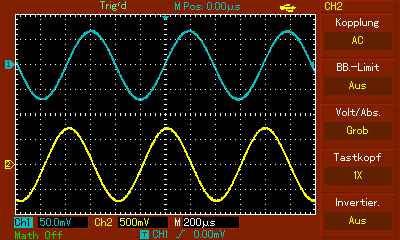
\includegraphics[width=\linewidth-70pt,height=\textheight-70pt,keepaspectratio]{content/MAP002.png}
	 	\label{fig:Sinus}
	 \end{figure}
	 In Abbildung 7 ist zu erkennen, dass die Spannung am Kondensator (blau) im Vergleich zur Spannung an der Spannungsquelle (gelb) um $\frac{\pi}{2}$ verschoben ist, was einer Integration der Sinus-Spannung an der Spannungsquelle mit einem Skalierungsfaktor entspricht. 
	 
	 
	 \begin{figure}[H]
	 	\centering
	 	\caption{}
	 	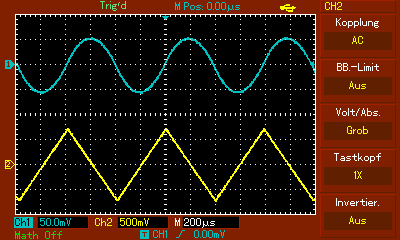
\includegraphics[width=\linewidth-70pt,height=\textheight-70pt,keepaspectratio]{content/MAP003.png}
	 	\label{fig:Dreieck}
	 \end{figure}
	 Auch bei Dreieckspannung an der Spannungsquelle (gelb) in Abbildung 8 lässt sich erkennen das die Spannung am Kondensator (blau) das Integral der Dreieckspannung ist, da die Kondensatorspannung sich wie bei einer Integration erwartet quardratisch verhält.
	 
	 \begin{figure}[H]
	 	\centering
	 	\caption{}
	 	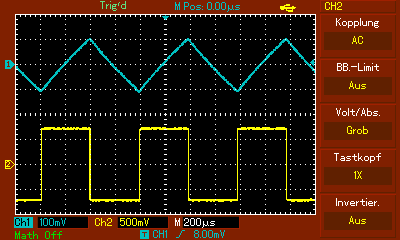
\includegraphics[width=\linewidth-70pt,height=\textheight-70pt,keepaspectratio]{content/MAP004.png}
	 	\label{fig:Rechteck}
	 \end{figure}
	 In Abbildung 9 beschreibt die Spannung an der Spannungsquelle eine Rechteckfunktion (gelb). Offensichtlich ist diese ein konstantes Vielfaches der Steigung der Kondensatorspannung (blau).
	 
	 Diese Beobachtungen bestätigen die Vermutung, dass der RC-Kreis auch als Integrator genutzt werden kann.
	 
